\chapter{Experiments}
\label{chp:4_results}
\section{Dataset}

We used the dataset and the provided model from NIPS 2017 Competition on Adversarial Attacks and Defenses~\cite{kurakin2018adversarial} to evaluate our method. NIPS 2017 dataset is a collection of 1000 images curated by Google Brain with a resolution of \(299 \times 299\) with their corresponding true and target classes from Imagenet~\cite{deng2009imagenet} dataset. For the target network, we used Inception-v3~\cite{szegedy2016rethinking} architecture and Imagenet trained checkpoint provided with the dataset.
\section{Experimental Evaluation}
We conducted our experiments in a white-box setup where the gradients are fully available. Experiments have been done in a targeted attack setting with the dataset provided targets. We optimized using Adam~\cite{kingma2015adam} with the default settings and used Carlini \& Wagner loss~\cite{carlini2017towards} with a confidence margin of \(\kappa \in \left\{ 0, 10 \right\}\).


\begin{table}[t]
    \caption{Average amount of distortion required to fool the target network with very high confidence (\(\kappa=10\)) in not restricted and subpixel restricted settings.}
    \label{table:perceptualmetrics}
    \begin{tabularx}{\linewidth}{ X  X  X  X }
        \toprule

                                           & RGB                               & \(C_{b}C_{r}\)                                             & \(a^*b^*\)                                \\
        \hline
        \multicolumn{4}{c}{Not Restricted}                                                                                                                                              \\
        \midrule
        LPIPS\newline SSIM\newline MS-SSIM & 0.327\newline 0.321\newline 0.164 & \textbf{0.019}\newline \textbf{0.067}\newline 0.017        & 0.022\newline 0.070\newline\textbf{0.016} \\
        \hline
        \multicolumn{4}{c}{Restricted to Subpixel}                                                                                                                                      \\
        \midrule
        LPIPS\newline SSIM\newline MS-SSIM & 0.222\newline 0.220\newline 0.037 & \textbf{0.012}\newline\textbf{0.050}\newline\textbf{0.011} & 0.014\newline 0.056\newline 0.013         \\
        \bottomrule
    \end{tabularx}
\end{table}

%\subsection{Results}
%\subsection{Fooling Rate and Success Rate}
We compared the success rate of our attack in CIELAB and \(YC_{b}C_{r}\) against stAdv in both restricted and unrestricted settings. An attack is considered successful if the Carlini \& Wagner loss is less than \(-\kappa\). We did not use the smoothness regularization term in stAdv for a fair comparison.
\begin{table}[t]
    \caption{Attack success rates with \(\kappa = 0\) and \(\kappa = 10\) in not restricted and subpixel restricted settings for RGB, \(a^*b^*\) and \(C_{b}C_{r}\) attacks. }

    \begin{tabularx}{\linewidth}{ X  X  X  X }
        \toprule
                                               & RGB                   & \(C_{b}C_{r}\)        & \(a^{*}b^{*}\)        \\
        \hline
        \multicolumn{4}{c}{Not Restricted}                                                                             \\
        \midrule
        \(\kappa\) = 0\newline \(\kappa\) = 10 & 100\%\newline 100\%   & 95.0\%\newline 83.8\% & 95.7\%\newline 87.3\% \\
        \hline
        \multicolumn{4}{c}{Restricted to Subpixel}                                                                     \\
        \midrule
        \(\kappa\) = 0\newline \(\kappa\) = 10 & 99.8\%\newline 99.7\% & 86.1\%\newline 47.0\% & 89.2\%\newline 53.2\% \\
        \bottomrule
    \end{tabularx}\label{table:foolingrate}
\end{table}


\begin{figure}[!b]

    \begin{subfigure}[b]{\linewidth}
        \caption{}

        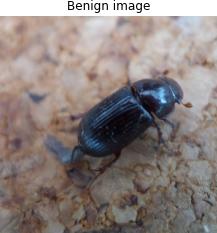
\includegraphics[width=0.24\linewidth]{examples/benign_0.png}
        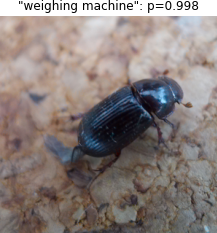
\includegraphics[width=0.24\linewidth]{examples/example_lab_0.png}
        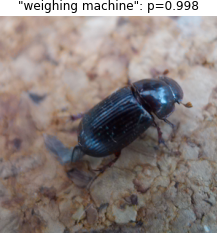
\includegraphics[width=0.24\linewidth]{examples/example_ycbcr_0.png}
        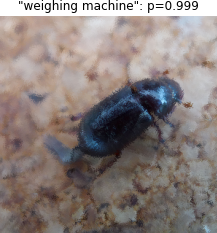
\includegraphics[width=0.24\linewidth]{examples/example_rgb_0.png}
    \end{subfigure}

    \begin{subfigure}[b]{\linewidth}
        \caption{}
        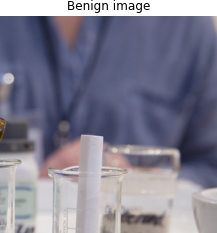
\includegraphics[width=0.24\linewidth]{examples/benign_4.png}
        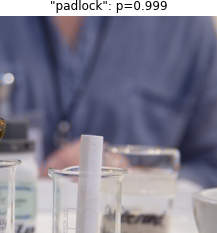
\includegraphics[width=0.24\linewidth]{examples/example_lab_4.png}
        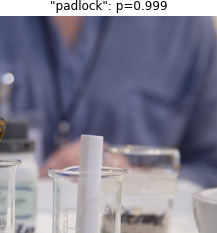
\includegraphics[width=0.24\linewidth]{examples/example_ycbcr_4.png}
        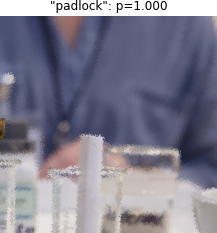
\includegraphics[width=0.24\linewidth]{examples/example_rgb_4.png}
    \end{subfigure}

    \begin{subfigure}[b]{\linewidth}
        \caption{}
        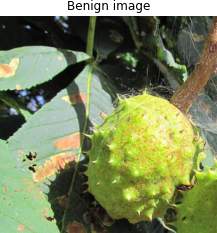
\includegraphics[width=0.24\linewidth]{examples/benign_5.png}
        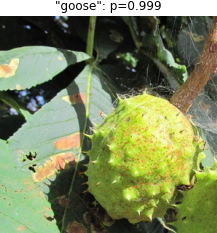
\includegraphics[width=0.24\linewidth]{examples/example_lab_5.png}
        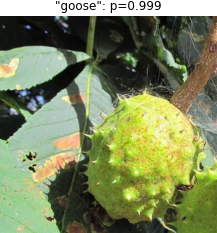
\includegraphics[width=0.24\linewidth]{examples/example_ycbcr_5.png}
        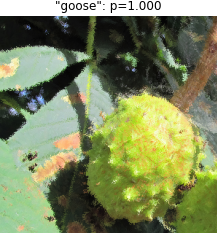
\includegraphics[width=0.24\linewidth]{examples/example_rgb_5.png}
    \end{subfigure}
\end{figure}

\begin{figure}[ht]
    \ContinuedFloat
    \begin{subfigure}[b]{\linewidth}
        \caption{}
        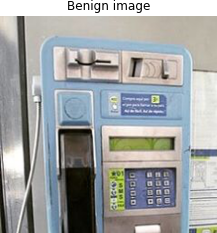
\includegraphics[width=0.24\linewidth]{examples/benign_20.png}
        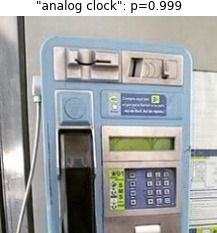
\includegraphics[width=0.24\linewidth]{examples/example_lab_20.png}
        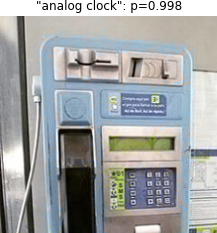
\includegraphics[width=0.24\linewidth]{examples/example_ycbcr_20.png}
        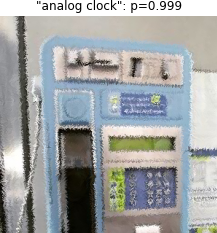
\includegraphics[width=0.24\linewidth]{examples/example_rgb_20.png}
    \end{subfigure}

    \begin{subfigure}[b]{\linewidth}
        \caption{}
        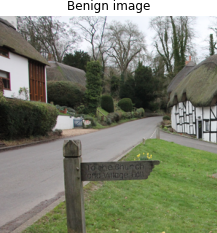
\includegraphics[width=0.24\linewidth]{examples/benign_7.png}
        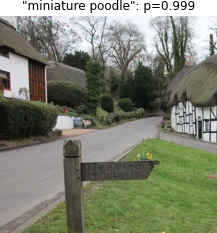
\includegraphics[width=0.24\linewidth]{examples/example_lab_7.png}
        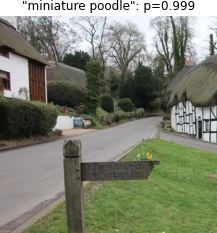
\includegraphics[width=0.24\linewidth]{examples/example_ycbcr_7.png}
        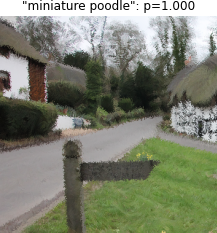
\includegraphics[width=0.24\linewidth]{examples/example_rgb_7.png}
    \end{subfigure}

    \begin{subfigure}[b]{\linewidth}
        \caption{}
        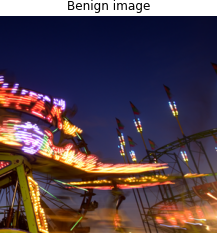
\includegraphics[width=0.24\linewidth]{examples/benign_30.png}
        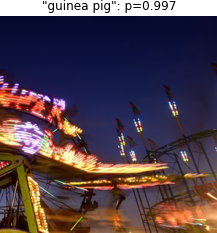
\includegraphics[width=0.24\linewidth]{examples/example_lab_30.png}
        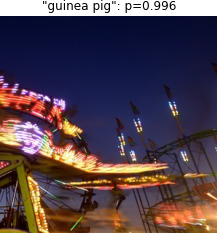
\includegraphics[width=0.24\linewidth]{examples/example_ycbcr_30.png}
        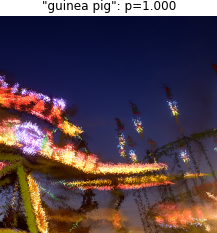
\includegraphics[width=0.24\linewidth]{examples/example_rgb_30.png}
    \end{subfigure}


    \caption[Examples from the dataset and adversarial examples generated with their target class probabilities from target network Inception-v3.]{Examples from the dataset and adversarial examples generated with their target class probabilities from target network Inception-v3. From left to right; Benign image, adversarial image generated by attacking to CbCr, a*b* and RGB channels. }\label{fig:visualprob}
\end{figure}

Figure~\ref{fig:visualprob} shows the original images alongside with the adversarial images generated (with \(\kappa = 10\)) by attacking in \(a^*b^*\), \(C_{b}C_{r}\) and RGB spaces. As can be observed from these images, perceptual distortions are much less pronounced for chrominance-only attacks. Attacking in RGB domain, which is the default approach in the literature, results in modification of the luminance channels, leading to much more visible artifacts.

Table~\ref*{table:foolingrate} shows the attack success rates for attacks on different colorspaces. The results show that, adversarial images generated by attacks exclusively targeting the chrominance channels can fool the network with a high probability as well. On the other hand, they are less effective when restricted to operate in a subpixel-only setting. The fooling rate of a*b* attacks are slightly higher than \(C_bC_r\) attacks. We argue that this is due to many examples in the dataset being chroma subsampled in \(YC_bC_r\) space, as an indirect effect of image compression, restricting the search space for \(C_bC_r\) attacks.

We measured the amount of distortion required to generate confident (\(\kappa = 10\)) adversarial examples with the following perceptual metrics: Learned Perceptual Image Patch Similarity~(LPIPS) ~\cite{zhang2018unreasonable}, Structured Similarity Index~(SSIM) ~\cite{wang2004image} and Multi-Scale SSIM~(MS-SSIM) ~\cite{wang2003multiscale}. Table~\ref{table:perceptualmetrics} shows the average results over the successful attacks for each perturbation mode in terms of these metrics. Since SSIM and MS-SSIM are similarity metrics, values of \(1-\)SSIM and \(1-\)MS-SSIM are provided. Hence, for all metrics, lower values are better. According to these results, colorspace restricted attacks have significantly better scores in terms of perceptual metrics compared to RGB attacks, implying that there is significantly less perceptual difference between benign and adversarial examples. While \(C_bC_r\) attacks generally produce better images in terms of perceptual quality metrics than a*b* attacks, the difference is relatively low.
